\chapter{Cryptanalysis of Hawk}
In this chapter we perform the cryptanalysis of Hawk. Note that we now switch notation so that $\vec{v}$ denotes a column vector to align with the notation and conventions of \cite{HawkSpec24}.
\section{Overview}

The original HPP attack can not work if the vector $\vec{x}$ multiplied with secret $\mat{V}$ has normally distributed entries as shown in section 3.4.
In Hawk, the distribution of entries of $\vec{x}$ is the \gls{dgd}. As the name implies, this distribution is discrete, not continuous. 
% The \gls{dgd} as described in \cite{HawkSpec24} / section 2.4 closely emulates
% that of its continuous normal counterpart, and the sampling procedure in the signature generation step in Hawk (see section 3.2...) 
% sample from \gls{dgd} using cumulative distribution tables.
Instead of showing theoretical and asymptotic results for the \gls{dgd}, we use our implementation of Hawk to measure and estimate the properties of the distribution.
The belief is that the discretization of the normal distribution in this manner makes the result in section 3.4 not hold in practice. 
Consequently, by applying the HPP attack on Hawk signatures one might be able to disclose the secret key.

The attack can be summarized as follows: 
\begin{algorithm}
\caption{HPP Hawk}
\begin{algorithmic}[1]
        \State Collect signatures $\vec{w} = \mat{B}^{-1} \vec{x}$
        \State Using public key $\mat{Q}$, find $\mat{L}$ s.t. $\mat{Q} = \mat{L} \mat{L}^t$
        \State Transform samples s.t. $\vec{c} = \mat{L}^t \vec{w}$
        \State Find columns of $\pm \mat{C}$ by doing gradient search over $\PP{C}$
        \State Multiply columns of $\pm \mat{C}$ by $\mat{L}^{-t}$ on the left to get columns in $\pm \mat{B}^{-1}$
\end{algorithmic}
\end{algorithm}

\begin{figure}[H]
    \centering
    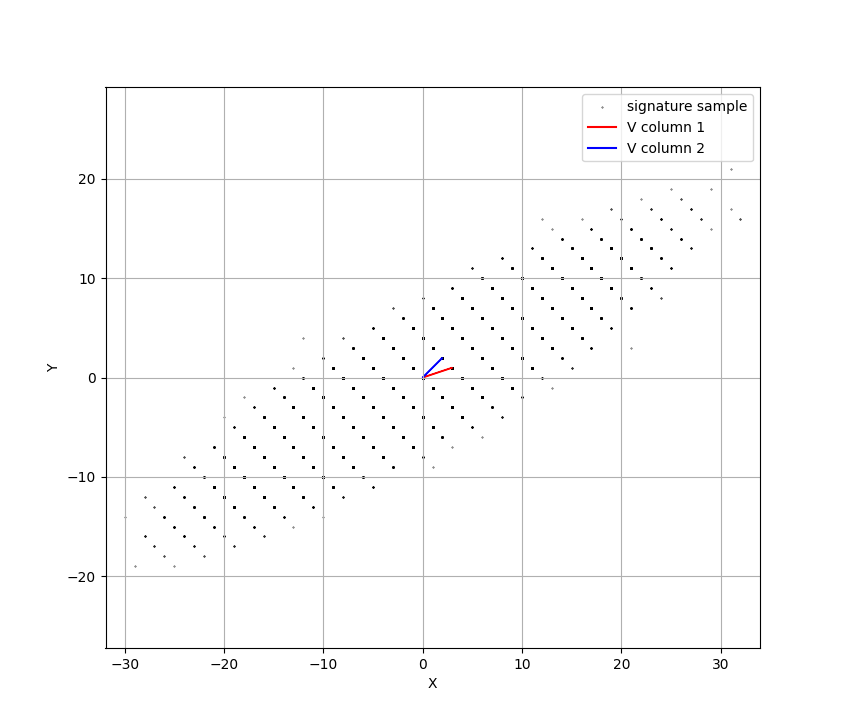
\includegraphics[scale=0.5]{hpp_parallelepiped_normal_discrete.png}
    \caption{Hidden parallelepiped problem in dimension 2 for rounded normal distribution}
  	\medskip 
	% \hspace*{15pt}\hbox{\scriptsize Credit: Acme company makes everything \url{https://acme.com/}}
    \label{parallelepiped_normal_discrete}
\end{figure}

\begin{figure}[H]
    \centering
    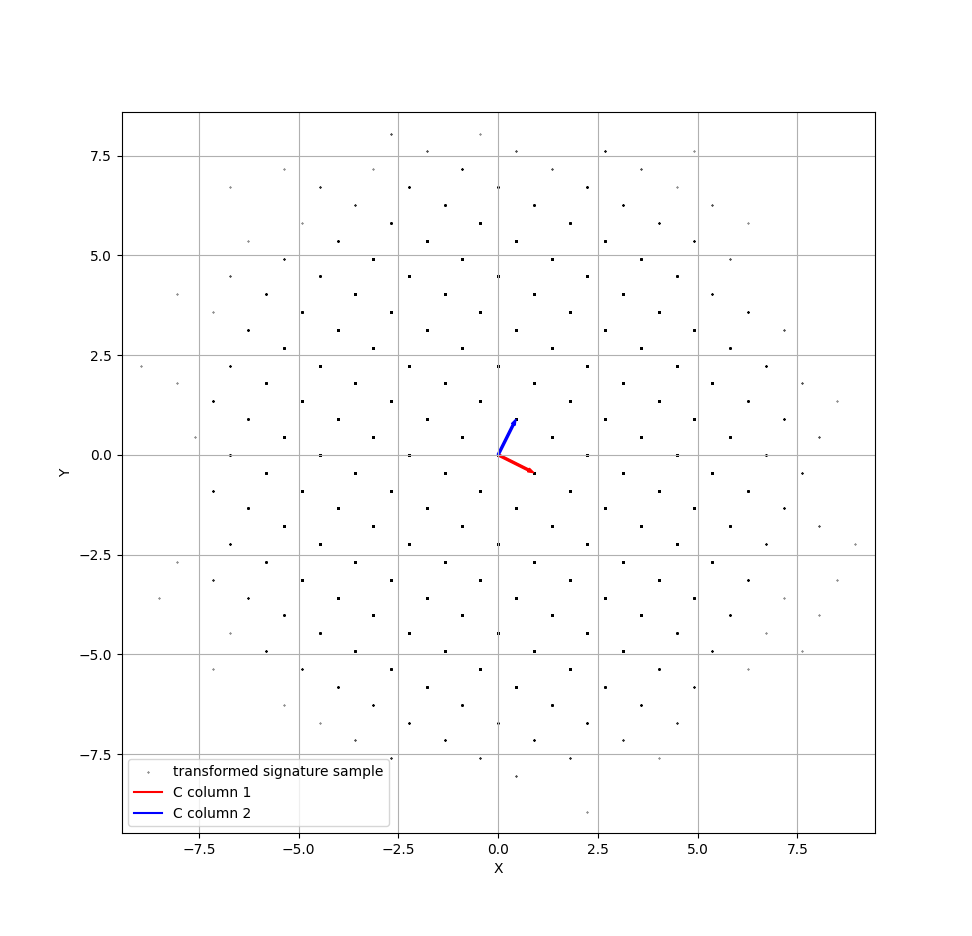
\includegraphics[scale=0.5]{hppnormal_cube_discrete.png}
    \caption{Hidden hypercube problem in dimension 2 for rounded normal distribution}
  	\medskip 
	% \hspace*{15pt}\hbox{\scriptsize Credit: Acme company makes everything \url{https://acme.com/}}
    \label{hypercube_normal_discrete}
\end{figure}
\section{HPP against practical Discrete Gaussian Distribution}
\subsection{Overview of method}
Consider the Discrete Gaussian Distribution as described in \cite{HawkSpec24} and in section 2.4... We use our implementation of Hawk to sample many points from the practical distribution.
Let $\dgd$ denote the theoretical discrete Gaussian distribution, and let $\dgdi$ denote the practical discrete Gaussian distribution from sampled points.
Let $0$, $\sigma^2$ be the expectation and variance of $\dgd$, and $\hat{\mu}$, $\hat{\sigma}^2$ be the expectation and variance of $\dgdi$.
Assume we sample $t$ points from $\dgdi$ as $X = \{x_1, x_2, ..., x_t\}$. We estimate $\hat{\mu}$ and $\hat{\sigma}^2$ simply as $\hat{\mu} = \mathlarger{\frac{1}{t} \sum_{i=1}^{t} x_i}$ and $\hat{\sigma}^2 = \mathlarger{\frac{1}{t} \sum_{i=1}^{t}(x_i - \hat{\mu})^2}$.
For simplicity, we can also assume $\hat{\mu} = \mu = 0$ as claimed in \cite{HawkSpec24}.
To simplify later computations we also normalize our samples by computing $Z = \{z_1, z_2, ..., z_t\} = \{\frac{x_1}{\hat{\sigma}}, \frac{x_2}{\hat{\sigma}},..., \frac{x_t}{\hat{\sigma}}\}$ such that 
$\bb{V}[z_i] = 1$.

% Note that as an attacker we can measure the properties of the distribution by observing $\vec{w}$. 

Now, denote by $\mu_4 = \bb{E}[z_i^4] = \mathlarger{\frac{1}{t} \sum_{i=1}^{n} z_i ^4}$. Assume observed signatures on the form $\vec{c} = \mat{C} \vec{z}$. By rewriting the terms from section 3.4 for this new, normalized, distribution $\dgdi$, we have that
\[mom_{4, \mat{C}} (\vec{w}) = 3 \lVert \vec{w} \rVert ^4 + (\mu_4 - 3) \sum_{i=1}^{n} \langle c_i, \vec{w} \rangle^4 \]
and
\todo{Maybe show more computations here}
\[\nabla mom_{4, \mat{C}} (\vec{w}) = 12 \lVert \vec{w} \rVert^2 \vec{w} + 4(\mu_4 - 3) \mathlarger{\sum_{i=1}^{n} \langle c_i, \vec{w}^3} \rangle c_i\]
This means that if the difference $(\mu_4 - 3)$ is big enough, one might be able to employ the same minimization technique as in the original attack to reveal a column of $\mat{V}$.
Note that if $(\mu_4 - 3) < 0$ we have the same case as in the original attack, where minimization of the entire term entails maximization of $\mathlarger{\sum_{i=1}^{n} \langle c_i, \vec{w} \rangle^4}$, which gives us a row of $\pm \mat{C}$.
If $(\mu_4 - 3) > 0$, we need to maximize the entire term $3 \lVert \vec{w} \rVert ^4 + \sum_{i=1}^{n} \langle c_i, \vec{w} \rangle^4$, which is achieved by doing a gradient \textit{ascent} instead of a gradient \textit{descent}.

\subsection{Covariance matrix and hypercube transformation}
In the original HPP attack one has to estimate the matrix $\mat{G} \approx \mat{V} ^t \mat{V}$ as $\vec{v} ^t \vec{v} \cdot 3$. We show that this is possible even if $x$ is normally distributed, as one can estimate 
$\frac{\vec{v}^t \vec{v}}{\sigma^2}$. For Hawk, the signatures are on the form $\vec{w} = \mat{B}^{-1} \vec{x}$. Then we would need to compute $\mat{G} = \mat{B}^{-1} \mat{B}^{-t} \approx \frac{\vec{w}\vec{w}^t}{\sigma^2}$.
In Hawk, however, the public key $\mat{Q} = \mat{B}^{*} \mat{B}$ which for columns $\vec{b} \in \bb{Q}^n$ is equivalent to $\mat{B} ^t \mat{B}$, enables us to skip this step.
Recall that in the original attack one has to take Cholesky decomposition (or an equivalent decomposition) of the inverse of the covariance matrix such that $\mat{G}^{-1} = \mat{L}\mat{L}^t$. For $\mat{G} = \mat{B}^{-1} \mat{B}^{-t}$, the inverse of $\mat{G}$,
$\mat{G}^{-1} = \mat{B}^t \mat{B} = \mat{Q}$. Therefore, we can simply take the Cholesky decomposition of $\mat{Q} = \mat{L} \mat{L}^t$.
By multiplying our samples $\vec{w}$ by $\mat{L}^t$ on the left, we have transformed our samples to the hidden hypercube as in the original attack. \\
By taking $\mat{C} =  \mat{L}^t\mat{B}^{-1}$, we have that 
\[\mat{C}^t \mat{C} = (\mat{L}^t \mat{B}^{-1})^t (\mat{L}^t \mat{B}^{-1}) = \mat{B}^{-t} \mat{L} \mat{L}^t \mat{B}^{-1} = \mat{B}^{-t} \mat{Q} \mat{B}^{-1} = \mat{B}^{-t} \mat{B}^{t} \mat{B} \mat{B}^{-1} = \mat{I}\]
and
\[\mat{C}\mat{C}^t = (\mat{L}^t \mat{B}^{-1})(\mat{L}^t \mat{B}^{-1})^t = \mat{L}^t \mat{B}^{-1} \mat{B}^{-t} \mat{L} =  \mat{L}^t \mat{Q}^{-1} \mat{L} = \mat{L}^t (\mat{L} \mat{L}^t)^{-1} \mat{L} = \mat{L}^t \mat{L}^{-t} \mat{L}^{-1} \mat{L} = \mat{I}\]
Since $\vec{x}$ is distributed according to $\dgdi$ over $\PP{\mat{B}^{-1}}$, by taking 
$\vec{c} = \mat{L}^{t} \vec{w}$ we have $\vec{c} = \mat{L}^{t} \mat{B}^{-1} \vec{x} = \mat{C} \vec{x}$, $\vec{c}$ is distributed according to $\dgdi$ over $\PP{C}$.

We summarize this step of the attack against Hawk in the following algorithm

\begin{algorithm}
\caption{Hawk Hypercube Transformation}
\begin{algorithmic}[1]
% \Procedure{Euclid}{$a,b$}\Comment{The g.c.d. of a and b}
    \Require{Samples $\vec{w} = \mat{B}^{-1} \vec{x}$ and public key $\mat{Q}$}
    \State Compute $\mat{L}$ s.t. $\mat{Q} = \mat{L}\mat{L}^t$ \Comment by Cholesky decomposition
    \State Compute $\vec{c} = \mat{L}^t \vec{w}$
    \State \Return{$\vec{c}$ and $\mat{L}^{-t}$}
\end{algorithmic}
\end{algorithm}

\subsection{Gradient search overview}
After having transformed the samples $\vec{w} \in \PP{\mat{B}^{-1}}$ to $\vec{c} \in \PP{\mat{C}}$ we want to recover columns of $\pm \mat{C}$ and transform them back to columns of $\pm \mat{B}^{-1}$ by multiplying by $\mat{L}^{-1}$ on the left.
Due to the special structure of Hawk (and NTRU) private keys, finding one column of $\mat{B}$, one has automatically found $n$ columns.
Unfortunately, since revealing a single column of $ \mat{B}^{-1}$ reveals a rotation of either the two polynomials $G$ and $ g$ \textit{or} $F$ and $f$,
this is not enough to disclose the entire matrix. If samples were on the form $\vec{w} = \mat{B} \vec{x}$, a single column would reveal $f$ and $g$, and one could simply reconstruct $F$ and $G$
by solving the NTRU-equation as in the key generation step of Hawk.
Nevertheless, if one finds two columns of $\mat{B}^{-1}$, it is easy to check if they are shifts of each other. If they are not, one has found shifts of all four polynomials in the secret key, 
and by trying all combinations of shifts, of which there are $4 n^2$ (accounting for negative and positive sign), one can easily verify if a candidate $\mat{B'}^{-1}$ is valid by computing 
$\mat{B'} = (\mat{B'}^{-1})^{-1}$, and checking if $\mat{B'}^t \mat{B'} = \mat{Q}$. If so, one is able to forge signatures, and the attack is done.

Now, given samples $\vec{c} \in \PP{C}$, we run a gradient search to minimize or maximize the fourth moment of one-dimensional projections, as in the original attack. In addition to multiplying the samples by $\mat{L}^t$, we also divide them by the scalar $\sigma$, to normalize the samples
so each sample in the vector $\vec{c}$ has variance $1$. This also aligns with our theoretical analysis of $\mom{4}{C}$. Even though the distribution $\dgdi$ is discrete, the shape of the samples $\vec{c} \in \PP{C}$ will still have a spherical
shape as illustrated in \ref{hypercube_normal_discrete}. The hope is that the areas in the directions of the columns of $\pm \mat{C}$ will deviate just enough from a perfect spherical shape to give us a global minima/maxima in the gradient landscape.

\subsection{Gradient search for Hawk}
Due to the noisy and unpredictable gradient landscape we need to search, the \textit{vanilla} gradient search method as used in the original HPP attack is not very good.
A constant stepsize means either a slow convergence (with a small value for $\delta$), or risking overshooting the correct extremum (with a big value for $\delta$).
Therefore, we employ a more advanced method for gradient search, namely the ADAM-optimizer \cite{KB17}.
